%!TeX root=../tese.tex

\chapter{Literatura Cinzenta}\label{cap:literatura-cinzenta}

Neste capítulo, estão apresentadas as fontes de literatura cinzenta utilizadas neste trabalho. Cada seção traz um resumo do conteúdo da fonte, seus resultados relevantes para este trabalho e um breve contexto da organização por trás dela.

\section{\citetitle{gitclear2025} \parencite*{gitclear2025}}

Este relatório foi escrito pela empresa GitClear, que desenvolve ferramentas de análise de código-fonte para empresas de desenvolvimento de software. O relatório realizou uma análise de métricas de qualidade de código de 211 milhões de linhas alteradas em 2024, sendo dois terços destas linhas advindos do compartilhamento de dados anonimizados de empresas privadas e o restante de projetos de código livre. Os pesquisadores criaram um histórico comparando as métricas observadas em pesquisas anteriores com as métricas de 2024 e a análise é feita com foco no impacto de ferramentas de IA generativa no processo de desenvolvimento de software, considerando 2022 como o ano em que a adoção da IA na programação se iniciou.

\begin{table}[h]
    \centering
    \footnotesize
    \caption{Histórico de métricas de código de 2020 a 2024 \parencite{gitclear2025}.}
    \label{tab:historico_metricas}
    \setlength{\tabcolsep}{6pt}
    \renewcommand{\arraystretch}{1.2}

    \begin{tabular}{llllllll}
        \toprule
        Ano    & Adicionado                  & Deletado    & Atualizado &
        Movido & Cópia                       & Substituído & Churn                                                                                                                      \\
        \midrule
        2020   & 39,2\%                      & 19,1\%      & 5,2\%      & 24,1\%                    & 8,3\%                     & 2,9\%                      & 3,1\%                    \\
        2021   & 39,5\%                      & 19,3\%      & 5,0\%      & 24,8\%                    & 8,4\%                     & 3,4\%                      & 3,3\%                    \\
        2022   & 40,9\%                      & 19,8\%      & 5,2\%      & \cellcolor{red!10} 20,5\% & 9,4\%                     & 3,7\%                      & 3,3\%                    \\
        2023   & \cellcolor{green!10} 42,3\% & 21,1\%      & 5,6\%      & \cellcolor{red!20} 15,8\% & \cellcolor{red!10} 10,6\% & \cellcolor{green!10} 3,6\% & \cellcolor{red!10} 4,5\% \\
        2024   & \cellcolor{green!20} 46,2\% & 21,9\%      & 5,9\%      & \cellcolor{red!30} 9,5\%  & \cellcolor{red!20} 12,3\% & \cellcolor{green!20} 4,2\% & \cellcolor{red!20} 5,7\% \\
        \bottomrule
    \end{tabular}
\end{table}

Na tabela \autoref{tab:historico_metricas}, são apresentados os resultados das análises entre 2020 e 2024. Observa-se que a porcentagem de linhas movidas, associada à refatoração, algo essencial para reduzir a dívida técnica e garantir a manutenibilidade do sistema a longo prazo, apresentou uma queda significativa, passando de 24,1\% em 2020 para apenas 9,5\% em 2024.

\begin{table}[h!]
    \centering
    \footnotesize
    \caption{Histórico de duplicação de código nos commits de 2020 a 2024 (\cite{gitclear2025}).}
    \label{tab:duplicacao_codigo}
    \setlength{\tabcolsep}{8pt}
    \renewcommand{\arraystretch}{1.2}
    \begin{tabular}{l l l l l}
        \toprule
        Ano                    &
        Tot. commits           &
        Tot. duplicações       &
        Commits com duplicação &
        Commits com duplicação (\%)                                     \\
        \midrule
        2020                   & 19{.}805 & 9{.}227  & 139     & 0,70\% \\
        2021                   & 29{.}912 & 9{.}295  & 143     & 0,48\% \\
        2022                   & 40{.}010 & 10{.}685 & 182     & 0,45\% \\
        2023                   & 41{.}561 & 20{.}448 & 747     & 1,80\% \\
        2024                   & 56{.}495 & 63{.}566 & 3{.}764 & 6,66\% \\
        \bottomrule
    \end{tabular}
\end{table}

Por outro lado, a tendência para as linhas copiadas foi inversa, partindo de 8,3\% em 2020 para 12,3\% em 2024. Este aumento de duplicações também pode ser observado na \autoref{tab:duplicacao_codigo}, que mostra que, em 2020, apenas 0,7\% dos commits analisados continham blocos de código duplicados e, em 2024, esse número subiu para 6,66\%. A duplicação de código, além de violar o princípio DRY (\emph{Don't Repeat Yourself}), segundo \citet{duplication_problems}, aumenta a probabilidade de erros no código, já que as cópias tendem a evoluir de forma inconsistente.

\begin{figure}[h!]
    \caption{Proporção anual das linhas modificadas classificadas pelo tempo que permaneceram no repositório antes de sofrerem uma nova modificação significativa entre 2020 e 2024 (\cite{gitclear2025}).}
    \centering
    \label{fig:historico_tempo_mudanca}

    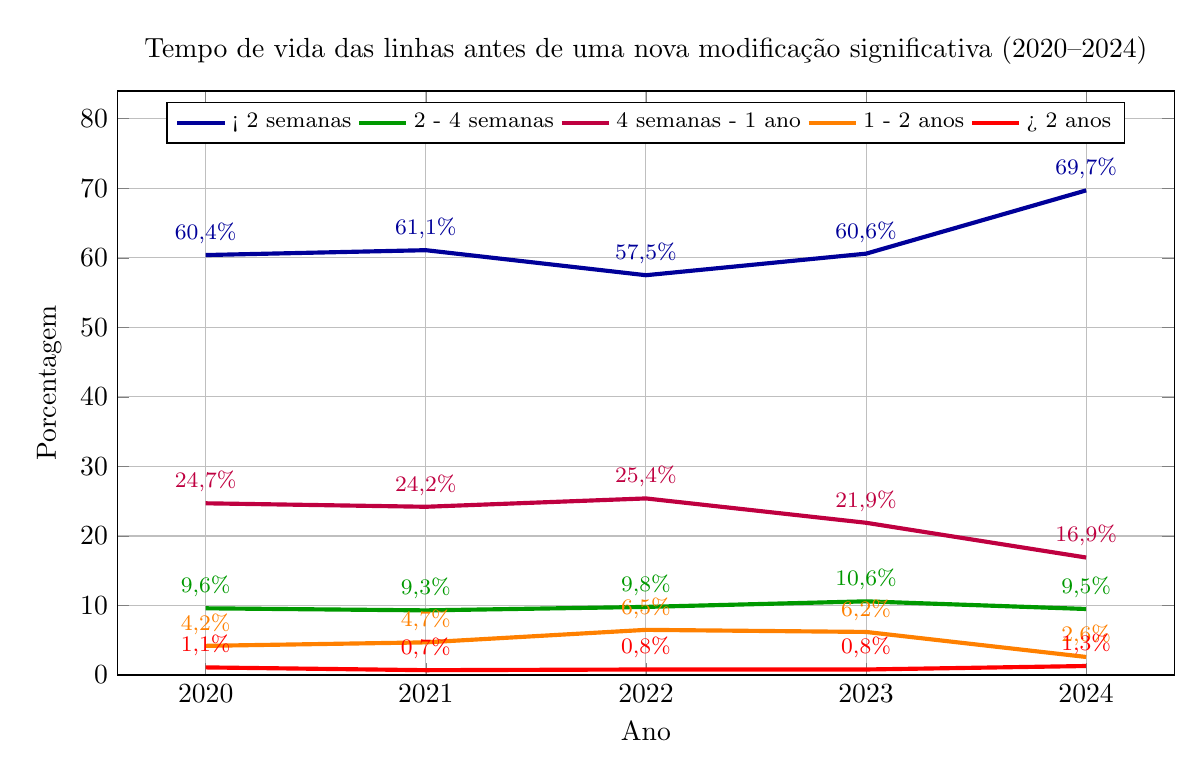
\begin{tikzpicture}
        \begin{axis}[
                /pgf/number format/use comma,
                every axis plot/.style={ line width=1.5pt },
                width=15cm,
                height=9cm,
                xlabel={Ano},
                ylabel={Porcentagem},
                title={Tempo de vida das linhas antes de uma nova modificação significativa (2020–2024)
                    },
                ymin=0,
                ymax=84,
                legend style={
                        font=\footnotesize,
                        at={(0.5,0.91)},
                        anchor=south,
                        legend columns=5,
                    },
                grid=both,
                symbolic x coords={2020,2021,2022,2023,2024},
                ytick distance=10,
                xtick=data,
                nodes near coords={\pgfmathprintnumber{\pgfplotspointmeta}\%},
                every node near coord/.append style={
                        font=\footnotesize,
                        anchor=south,
                    },
            ]

            \addplot[color=blue!60!black] coordinates {
                    (2020,60.4) (2021,61.1) (2022,57.5) (2023,60.6) (2024,69.7)
                };
            \addlegendentry{< 2 semanas}

            \addplot[color=green!60!black] coordinates {
                    (2020,9.6) (2021,9.3) (2022,9.8) (2023,10.6) (2024,9.5)
                };
            \addlegendentry{2 - 4 semanas}

            \addplot[color=purple] coordinates {
                    (2020,24.7) (2021,24.2) (2022,25.4) (2023,21.9) (2024,16.9)
                };
            \addlegendentry{4 semanas - 1 ano}

            \addplot[color=orange] coordinates {
                    (2020,4.2) (2021,4.7) (2022,6.5) (2023,6.2) (2024,2.6)
                };
            \addlegendentry{1 - 2 anos}

            \addplot[color=red] coordinates {
                    (2020,1.1) (2021,0.7) (2022,0.8) (2023,0.8) (2024,1.3)
                };
            \addlegendentry{> 2 anos}

        \end{axis}
    \end{tikzpicture}

\end{figure}

Observa-se também um aumento de 2,9\% para 4,2\% entre 2020 e 2024 na proporção de linhas substituídas. O relatório credita essa mudança ao uso de IDEs e assistentes de código de IA, que podem com facilidade reescrever trechos de código para conformar-se às regras de linting e às convenções do projeto.

Além disso, outra métrica relevante neste contexto é o \emph{churn}, que busca medir quanto retrabalho é efetuado em uma base de código. Neste relatório, o \emph{churn} é calculado medindo quanto das linhas escritas e enviadas ao repositório foram revertidas ou substancialmente revisadas nas duas semanas seguintes. A \autoref{tab:historico_metricas} mostra que o \emph{churn} passou de 3,1\% em 2020 para 5,7\% em 2024, evidenciando o aumento do retrabalho no código.

O relatório fez também uma análise de quanto tempo se passou entre o momento em que os códigos analisados foram criados e em quanto tempo eles receberam sua próxima mudança significativa. Na \autoref{fig:historico_tempo_mudanca}, observa-se que a proporção de linhas que em menos de duas semanas foram alteradas aumentou de 60,4\% em 2020 para 69,7\% em 2024, em contrapartida, o grupo das linhas que precisaram de alterações apenas depois de 4 semanas, mas antes de um ano, diminuiu de 24,7\% para 16,9\% no mesmo período.

\section{\citetitle{StackOverflow2023} \parencite*{StackOverflow2023,StackOverflow2024,StackOverflow2025}}

Esta seção compila os resultados de 3 anos da \emph{Stack Overflow Developer Survey} de 2023 a 2025. Esta pesquisa é realizada anualmente pela \emph{Stack Overflow}, uma das principais plataformas \emph{online} de perguntas e respostas voltadas para desenvolvedores de \emph{software}, que possibilita que programadores de todo o mundo tirem dúvidas técnicas, compartilhem soluções e aprendam a partir de problemas reais.

A pesquisa é aberta, incluindo respondentes de todo o mundo, desde programadores profissionais até pessoas que estão iniciando seus estudos sobre programação. A pesquisa coleta dados sobre o uso de tecnologias, linguagens de programação, ferramentas, práticas de desenvolvimento, perfil profissional e, mais recentemente, uso de IA no processo de desenvolvimento de \emph{software}. Os resultados das perguntas geralmente permitem fazer o recorte dos respondentes quanto ao seu conhecimento de programação, as respostas dadas por programadores profissionais foram priorizadas nesta seção.

\begin{figure}[h!]
    \caption{Proporção anual dos desenvolvedores profissionais que utilizam ferramentas de IA em seu processo de desenvolvimento entre 2023 e 2025 (\cite{StackOverflow2023}; \cite*{StackOverflow2024,StackOverflow2025}; n\textsubscript{2023} = 67237; n\textsubscript{2024} =  46049; n\textsubscript{2025} = 33662).}
    \label{fig:historico_uso_ia}
    \centering
    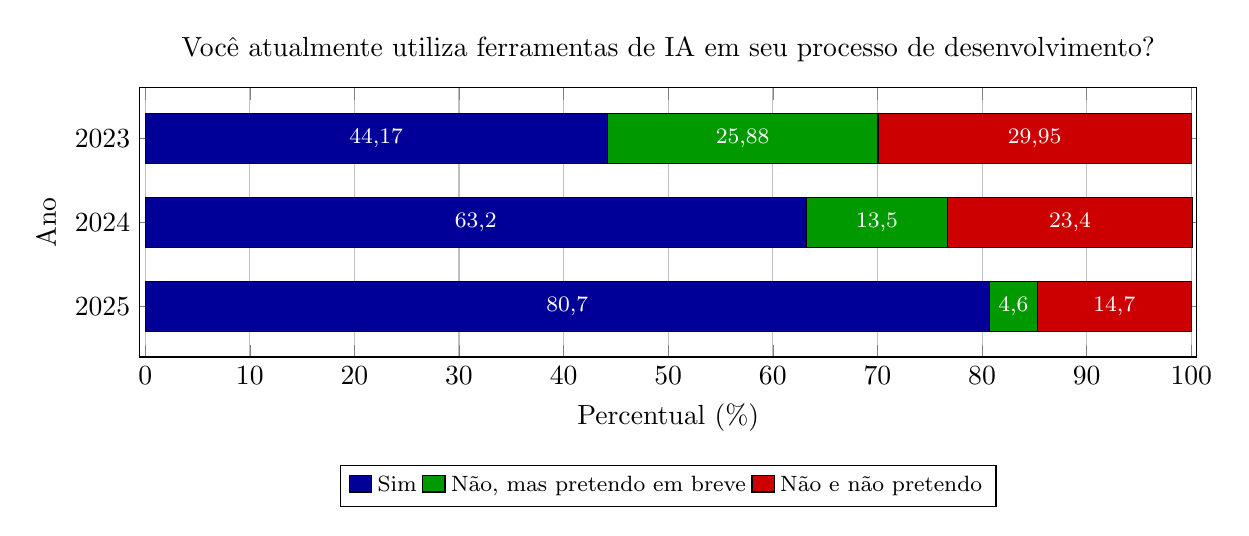
\begin{tikzpicture}
        \begin{axis}[
                /pgf/number format/use comma,
                xbar stacked,
                width=15cm,
                height=5cm,
                title={Você atualmente utiliza ferramentas de IA em seu processo de desenvolvimento?},
                xlabel={Percentual (\%)},
                ylabel={Ano},
                xmin=0, xmax=100,
                symbolic y coords={2023,2024,2025},
                ytick=data,
                y dir=reverse,
                enlarge y limits=0.3,
                xtick distance=10,
                grid=both,
                bar width=18pt,
                nodes near coords,
                nodes near coords align={center},
                nodes near coords style={
                        font=\footnotesize\bfseries,
                        color=white
                    },
                enlarge x limits=0.005,
                legend style={
                        font=\footnotesize,
                        at={(0.5,-0.4)},
                        anchor=north,
                        legend columns=3,
                    },
            ]

            % Sim
            \addplot[fill=blue!60!black] coordinates {
                    (44.17,2023)
                    (63.2,2024)
                    (80.7,2025)
                };
            \addlegendentry{Sim}

            % Não, mas pretendo em breve
            \addplot[fill=green!60!black] coordinates {
                    (25.88,2023)
                    (13.5,2024)
                    (4.6,2025)
                };
            \addlegendentry{Não, mas pretendo em breve}

            % Não e não pretendo
            \addplot[fill=red!80!black] coordinates {
                    (29.95,2023)
                    (23.4,2024)
                    (14.7,2025)
                };
            \addlegendentry{Não e não pretendo}

        \end{axis}
    \end{tikzpicture}
\end{figure}

Na \autoref{fig:historico_uso_ia}, estão apresentados os dados referentes à adoção de ferramentas de IA por parte dos desenvolvedores profissionais que participaram das pesquisas ao longo dos três anos. O gráfico captura o forte crescimento na adoção destas ferramentas, partindo de 44,17\% de uso em 2023 para 80,7\% em 2025.

\begin{figure}[h!]
    \caption{Proporção anual da percepção dos desenvolvedores profissionais em relação às ferramentas de IA de 2023 a 2025 (\cite{StackOverflow2023}; \cite*{StackOverflow2024,StackOverflow2025}; n\textsubscript{2023} = 46928; n\textsubscript{2024} =  35142; n\textsubscript{2025} = 25814).}
    \label{fig:percepcao_ia}
    \centering
    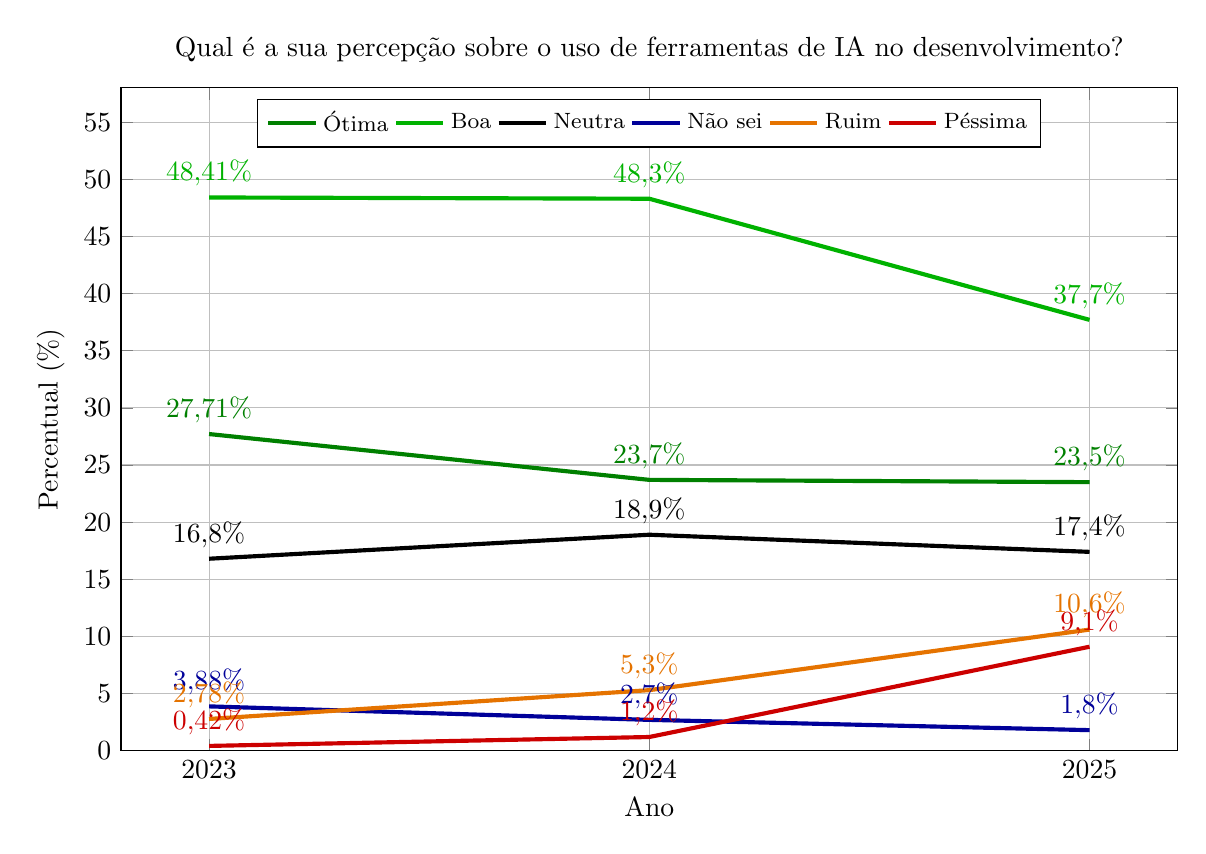
\begin{tikzpicture}
        \begin{axis}[
                /pgf/number format/use comma,
                width=15cm,
                height=10cm,
                title={Qual é a sua percepção sobre o uso de ferramentas de IA no desenvolvimento?},
                xlabel={Ano},
                ylabel={Percentual (\%)},
                ymin=0, ymax=58,
                symbolic x coords={2023,2024,2025},
                xtick=data,
                ytick distance=5,
                grid=both,
                nodes near coords={\pgfmathprintnumber{\pgfplotspointmeta}\%},
                every axis plot/.style={ line width=1.5pt },
                legend style={
                        font=\footnotesize,
                        at={(0.5,0.91)},
                        anchor=south,
                        legend columns=6,
                    },
            ]

            % Very favorable
            \addplot[color=green!50!black] coordinates {
                    (2023,27.71)
                    (2024,23.7)
                    (2025,23.5)
                };
            \addlegendentry{Ótima}

            % Favorable
            \addplot[color=green!70!black] coordinates {
                    (2023,48.41)
                    (2024,48.3)
                    (2025,37.7)
                };
            \addlegendentry{Boa}

            % Indifferent
            \addplot[color=black] coordinates {
                    (2023,16.8)
                    (2024,18.9)
                    (2025,17.4)
                };
            \addlegendentry{Neutra}

            % Unsure
            \addplot[color=blue!60!black] coordinates {
                    (2023,3.88)
                    (2024,2.7)
                    (2025,1.8)
                };
            \addlegendentry{Não sei}

            % Unfavorable
            \addplot[color=orange!90!black] coordinates {
                    (2023,2.78)
                    (2024,5.3)
                    (2025,10.6)
                };
            \addlegendentry{Ruim}

            % Very unfavorable
            \addplot[color=red!80!black] coordinates {
                    (2023,0.42)
                    (2024,1.2)
                    (2025,9.1)
                };
            \addlegendentry{Péssima}

        \end{axis}
    \end{tikzpicture}
\end{figure}

Na \autoref{fig:percepcao_ia}, estão apresentados os dados referentes à percepção dos desenvolvedores sobre uso de IA no desenvolvimento de \emph{software}. As impressões dos programadores têm mudado de pesquisa para pesquisa. De 2023 a 2025, as porcentagens de profissionais que têm uma percepção boa ou ótima sobre as ferramentas de IA caíram de 48,41\% para 37,7\% e de 27,71\% para 23,5\%, respectivamente. Por outro lado, no mesmo período, as percepções ruim e péssima subiram de 2,78\% para 10,6\% e de 0,42\% para 9,1\%, respectivamente. A mudança fica ainda mais evidente ao agrupar as percepções positivas e negativas, já que as positivas caíram de 76,12\% para 61,2\% e as negativas subiram de 3,2\% para 19,7\%, um crescimento bastante expressivo.

\begin{figure}[h!]
    \caption{Proporção anual do nível de confiança dos desenvolvedores em ferramentas de IA entre 2023 e 2025 (\cite{StackOverflow2023}; \cite*{StackOverflow2024,StackOverflow2025}; n\textsubscript{2023} = 39042; n\textsubscript{2024} =  28829; n\textsubscript{2025} = 25701).}
    \label{fig:confianca_ia}
    \centering
    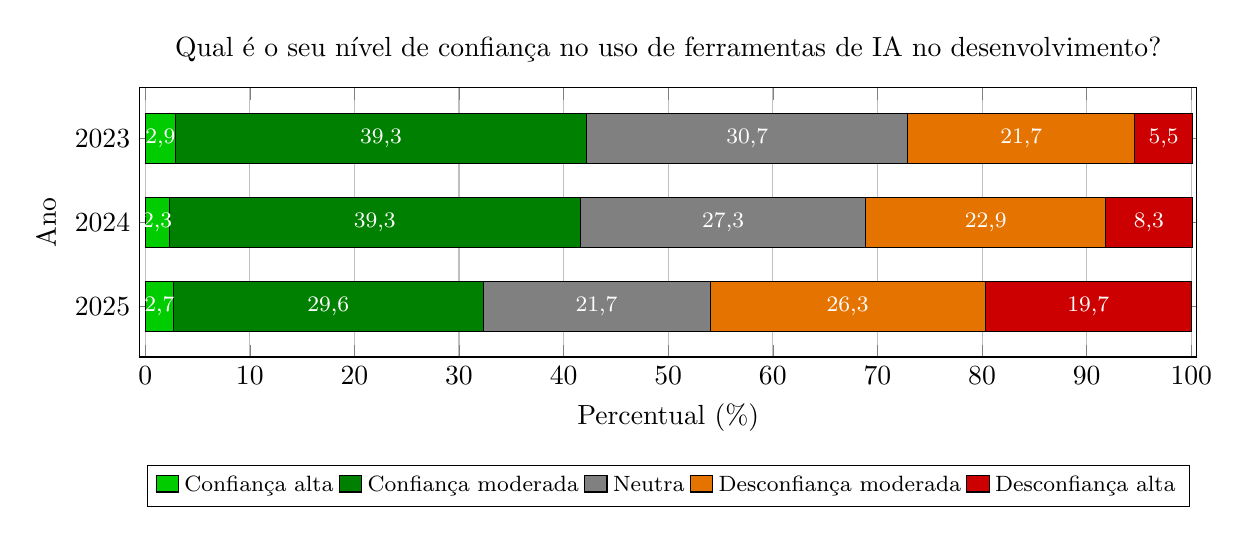
\begin{tikzpicture}
        \begin{axis}[
                /pgf/number format/use comma,
                xbar stacked,
                width=15cm,
                height=5cm,
                title={Qual é o seu nível de confiança no uso de ferramentas de IA no desenvolvimento?},
                xlabel={Percentual (\%)},
                ylabel={Ano},
                xmin=0, xmax=100,
                symbolic y coords={2023,2024,2025},
                ytick=data,
                y dir=reverse,
                enlarge y limits=0.3,
                xtick distance=10,
                grid=both,
                bar width=18pt,
                nodes near coords,
                nodes near coords align={center},
                nodes near coords style={
                        font=\footnotesize\bfseries,
                        color=white
                    },
                enlarge x limits=0.005,
                legend style={
                        font=\footnotesize,
                        at={(0.5,-0.4)},
                        anchor=north,
                        legend columns=5,
                    },
            ]

            % Confiança muito alta
            \addplot[fill=green!80!black] coordinates {
                    (2.9,2023)
                    (2.3,2024)
                    (2.7,2025)
                };
            \addlegendentry{Confiança alta}

            % Confiança moderada
            \addplot[fill=green!50!black] coordinates {
                    (39.3,2023)
                    (39.3,2024)
                    (29.6,2025)
                };
            \addlegendentry{Confiança moderada}

            % Neutra
            \addplot[fill=gray] coordinates {
                    (30.7,2023)
                    (27.3,2024)
                    (21.7,2025)
                };
            \addlegendentry{Neutra}

            % Desconfiança moderada
            \addplot[fill=orange!90!black] coordinates {
                    (21.7,2023)
                    (22.9,2024)
                    (26.3,2025)
                };
            \addlegendentry{Desconfiança moderada}

            % Desconfiança muito alta
            \addplot[fill=red!80!black] coordinates {
                    (5.5,2023)
                    (8.3,2024)
                    (19.7,2025)
                };
            \addlegendentry{Desconfiança alta}

        \end{axis}
    \end{tikzpicture}
\end{figure}

Seguindo a tendência de piora, a \autoref{fig:confianca_ia} apresenta o grau de confiança dos programadores em relação aos resultados apresentados pelas ferramentas de IA. De 2023 a 2025, as proporções de profissionais com confiança moderada ou alta em ferramentas de IA caíram de 39,3\% para 29,6\% e de 2,85\% para 2,7\%, respectivamente. Em contrapartida, no mesmo período, as desconfianças moderada e alta subiram de 21,71\% para 26,3\% e de 5,46\% para 19,7\%, respectivamente. Como no dado anterior, agrupar os graus positivos e negativos evidencia a queda, já que a confiança foi de 42,15\% para 32,3\%, enquanto a desconfiança subiu de 27,17\% para 46\%, ou seja, em 2025, menos respondentes confiam nas ferramentas de IA que o contrário.

\begin{figure}[h!]
    \centering
    \caption{Percepção dos desenvolvedores profissionais sobre a capacidade das ferramentas de IA em lidar com tarefas complexas em 2025 (\cite{StackOverflow2025}; n = 25695).}

    Quão bem as ferramentas de IA que você usa em seu fluxo de trabalho de desenvolvimento lidam com tarefas complexas?
    \vspace{0.5cm}

    \label{fig:ia_tarefas_complexas_2025}
    \begin{tikzpicture}
        \pie[
            radius=3,
            text=legend,
            sum=100,
            after number=\%,
            color={
                green!60!black,
                green!80!black,
                gray,
                orange!100!black,
                red!80!white,
                blue!60!white,
                blue!60!black
            }
        ]{3.9/{Muito bem}, 25.2/{Bem, mas não perfeitamente}, 14.2/{Nem bem nem mal}, 22.8/{Mal}, 18.6/{Muito mal}, 15.3/{Não sei/não utilizo para isso}}
    \end{tikzpicture}
\end{figure}

A \autoref{fig:ia_tarefas_complexas_2025} mostra a percepção dos desenvolvedores profissionais em 2025 em relação à capacidade das ferramentas de IA em lidar com tarefas complexas. Embora cerca de 29,1\% dos respondentes avaliem o desempenho como positivo, uma parcela significativa considera o desempenho como insatisfatório, com cerca de 41\% classificando-a como mal ou muito mal. Esses resultados indicam que, apesar dos avanços, ainda há limitações relevantes no uso de IA para atividades de maior complexidade no desenvolvimento de software. Este gráfico trouxe apenas os dados de 2025 porque a pergunta não foi feita em 2023 e em 2024, as alternativas para resposta mudaram, dificultando a comparação entre anos.

\begin{figure}[h!]
    \caption{Uso atual e interesse futuro no uso de ferramentas de IA ao longo do fluxo de desenvolvimento em 2024 (\cite{StackOverflow2024}; n = 35978)}
    \label{fig:uso_ia_fluxo_desenvolvimento}
    \centering
    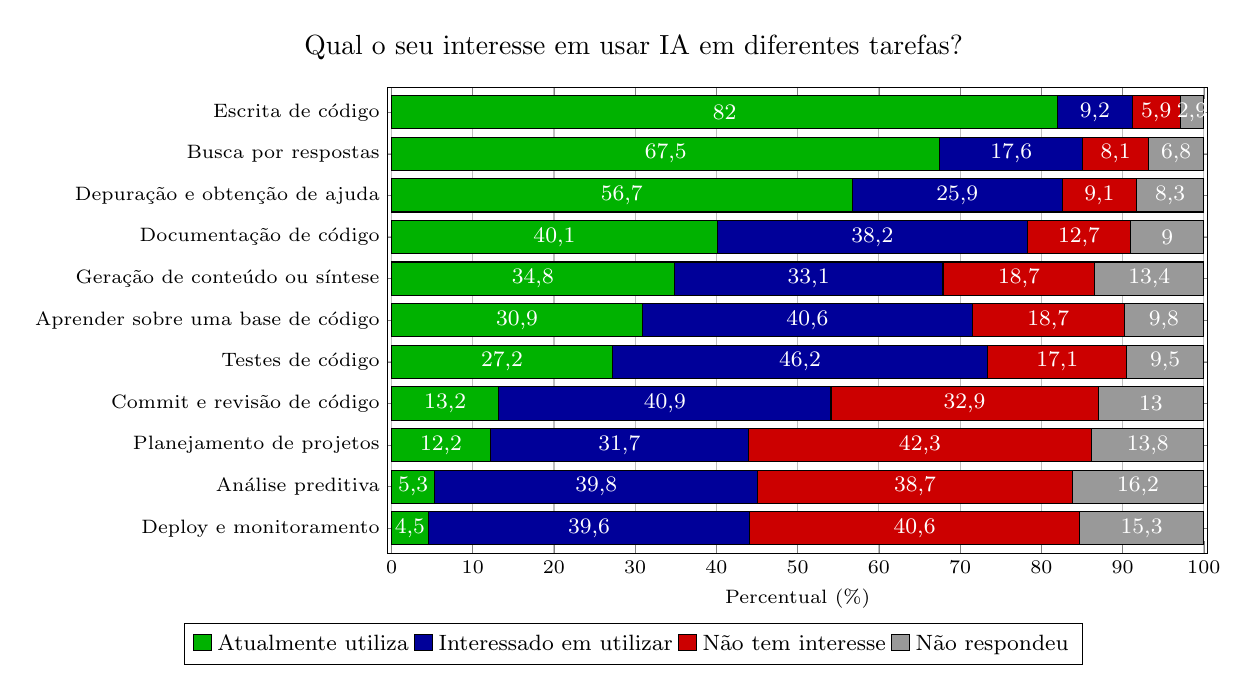
\begin{tikzpicture}
        \scriptsize
        \begin{axis}[
            /pgf/number format/use comma,
            xbar stacked,
            width=12cm,
            height=7.5cm,
            title={Qual o seu interesse em usar IA em diferentes tarefas?},
            title style={at={(0.3,1.05)}, anchor=center, font=\normalsize},
            xlabel={Percentual (\%)},
            xmin=0, xmax=100,
            symbolic y coords={
                Escrita de código,
                Busca por respostas,
                Depuração e obtenção de ajuda,
                Documentação de código,
                Geração de conteúdo ou síntese,
                Aprender sobre uma base de código,
                Testes de código,
                Commit e revisão de código,
                Planejamento de projetos,
                Análise preditiva,
                Deploy e monitoramento
            },
            ytick=data,
            y dir=reverse,
            enlarge y limits=0.06,
            xtick distance=10,
            grid=both,
            bar width=12pt,
            nodes near coords,
            nodes near coords align={center},
            nodes near coords style={
                font=\footnotesize\bfseries,
                color=white
            },
            enlarge x limits=0.005,
            legend style={
                font=\footnotesize,
                at={(0.3,-0.15)},
                anchor=north,
                legend columns=4,
            },
        ]

        % Atualmente usa
        \addplot[fill=green!70!black] coordinates {
            (82.0,Escrita de código)
            (67.5,Busca por respostas)
            (56.7,Depuração e obtenção de ajuda)
            (40.1,Documentação de código)
            (34.8,Geração de conteúdo ou síntese)
            (30.9,Aprender sobre uma base de código)
            (27.2,Testes de código)
            (13.2,Commit e revisão de código)
            (12.2,Planejamento de projetos)
            (5.3,Análise preditiva)
            (4.5,Deploy e monitoramento)
        };
        \addlegendentry{Atualmente utiliza}

        % Interessado em usar
        \addplot[fill=blue!60!black] coordinates {
            (9.2,Escrita de código)
            (17.6,Busca por respostas)
            (25.9,Depuração e obtenção de ajuda)
            (38.2,Documentação de código)
            (33.1,Geração de conteúdo ou síntese)
            (40.6,Aprender sobre uma base de código)
            (46.2,Testes de código)
            (40.9,Commit e revisão de código)
            (31.7,Planejamento de projetos)
            (39.8,Análise preditiva)
            (39.6,Deploy e monitoramento)
        };
        \addlegendentry{Interessado em utilizar}

        % Não interessado
        \addplot[fill=red!80!black] coordinates {
            (5.9,Escrita de código)
            (8.1,Busca por respostas)
            (9.1,Depuração e obtenção de ajuda)
            (12.7,Documentação de código)
            (18.7,Geração de conteúdo ou síntese)
            (18.7,Aprender sobre uma base de código)
            (17.1,Testes de código)
            (32.9,Commit e revisão de código)
            (42.3,Planejamento de projetos)
            (38.7,Análise preditiva)
            (40.6,Deploy e monitoramento)
        };
        \addlegendentry{Não tem interesse}

        % Não respondeu
        \addplot[fill=gray!80] coordinates {
            (2.9,Escrita de código)
            (6.8,Busca por respostas)
            (8.3,Depuração e obtenção de ajuda)
            (9.0,Documentação de código)
            (13.4,Geração de conteúdo ou síntese)
            (9.8,Aprender sobre uma base de código)
            (9.5,Testes de código)
            (13,Commit e revisão de código)
            (13.8,Planejamento de projetos)
            (16.2,Análise preditiva)
            (15.3,Deploy e monitoramento)
        };
        \addlegendentry{Não respondeu}
        \end{axis}
    \end{tikzpicture}
\end{figure}

A \autoref{fig:uso_ia_fluxo_desenvolvimento} apresenta os principais usos que os programadores têm feito das ferramentas de IA em 2024. O gráfico mostra que as atividades para as quais os desenvolvedores mais estão utilizando IA são: escrita de código (82\%), busca por respostas (67,5\%) e depuração e obtenção de ajuda (56,7\%). Por outro lado, as tarefas para as quais os desenvolvedores estão menos interessados em utilizar IA são: planejamento de projetos (42,3\%), implantação e monitoramento (40,6\%) e análise preditiva (38,7\%). Este gráfico inclui apenas os dados de 2024, pois, em 2023, a pergunta permitia respostas de modo que as categorias de uso e interesse se sobrepunham e, em 2025, havia mais categorias possíveis, incluindo "usa majoritariamente IA", "parcialmente IA", entre outros, dificultando a comparação com anos anteriores. 

\begin{table}[h!]
\centering
\caption{Proporção de desenvolvedores que não têm interesse em utilizar ferramentas de IA em diferentes partes do SDLC entre 2023 e 2025. As atividades presentes em apenas uma das pesquisas não foram incluídas (\cite{StackOverflow2023}; \cite*{StackOverflow2024,StackOverflow2025}; n\textsubscript{2023} = 37726; n\textsubscript{2024} =  35978; n\textsubscript{2025} = 25349).}
\label{tab:nao_interesse_ia}
\begin{tabular}{lccc}
\toprule
\textbf{Atividade} & \textbf{2023 (\%)} & \textbf{2024 (\%)} & \textbf{2025 (\%)} \\
\midrule

\emph{Deploy} e monitoramento           & 28,3 & 40,6 & 75,8 \\
Planejamento de projetos                & 29,8 & 42,3 & 69,2 \\
Análise preditiva                       & -    & 38,7 & 65,6 \\
Commit e revisão de código              & 23,0 & 32,9 & 58,7 \\
Testes de código                        & 11,4 & 17,1 & 44,1 \\
Aprender sobre uma base de código       & 13,1 & 18,7 & 39,4 \\
Documentação de código                  & 8,1  & 12,7 & 38,5 \\
Geração de conteúdo ou dados sintéticos & -    & 18,7 & 38,2 \\
Depuração ou correção de código         & 6,4  & 9,1  & 36,4 \\
Escrita de código                       & 4,5  & 5,9  & 28,9 \\
Busca por respostas                     & -    & 8,1  & 19,6 \\
\bottomrule
\end{tabular}
\end{table}

Apesar disso, a categoria que cobre o fato dos respondentes não terem interesse em usar IA para uma determinada tarefa está presente nas três pesquisas. Na \autoref{tab:nao_interesse_ia}, está compilado o histórico dessa categoria de 2023 a 2025 e a tendência para todas as atividades foi de diminuição do interesse no uso de IA. \emph{Deploy} e monitoramento e planejamento de projetos foram as tarefas com as maiores porcentagens, 75,8\% e 69,2\%, ou seja, a maioria dos programadores não tem interesse em usar IA nelas. 

\section{\citetitle{gartner_ai_code_assistants_2024} \parencite*{gartner_ai_code_assistants_2024}}

Este relatório foi produzido por pesquisadores da \emph{Gartner Research}. A \emph{Gartner} é uma empresa de pesquisa e consultoria especializada em tecnologia da informação e gestão empresarial, fundada em 1979. A organização é reconhecida pela produção de relatórios analíticos, previsões de mercado e estudos prospectivos sobre tendências tecnológicas, amplamente utilizados por empresas e organizações como suporte à tomada de decisão estratégica.

Neste relatório, há uma análise de diferentes aspectos relativos aos assistentes de código baseados em IA. As previsões do relatório sobre essas ferramentas são:

\begin{itemize}
    \item De 2024 até 2027, o número de equipes de engenharia de plataforma que utilizarão IA para aprimorar todas as fases do SDLC aumentará de 5\% para 40\%;
    \item Até 2027, 80\% das empresas integrarão ferramentas de teste com IA em sua cadeia de produção de \emph{software}, representando um aumento significativo em relação a cerca de 15\% no início de 2023;
    \item Até 2027, 25\% dos defeitos de \emph{software} que chegarão ao ambiente de produção resultarão da falta de supervisão humana sobre código gerado por IA, um aumento expressivo em comparação com menos de 1\% em 2023;
    \item Até 2028, 90\% dos engenheiros de \emph{software} em ambientes corporativos utilizarão assistentes de código baseados em IA, frente a menos de 14\% no início de 2024;
    \item Até 2028, o uso de IA generativa reduzirá em 30\% os custos de modernização de aplicações legadas em relação aos níveis de 2023.
\end{itemize}

As previsões do relatório apontam para a continuidade da tendência de adoção de IA generativa na engenharia de \emph{software}. Além disso, o texto destaca vantagens dessas ferramentas, como poder aprimorar a experiência do desenvolvedor de \emph{software} ao impulsionar o desenvolvimento de aplicações, minimizar a sobrecarga cognitiva dos programadores, ampliar suas habilidades de resolução de problemas, acelerar o ritmo de aprendizado e fomentar a criatividade.

Outro ponto levantado pelo relatório são as funcionalidades essenciais para que essas ferramentas atendam às necessidades de mercado, as funcionalidades são:

\begin{itemize}
    \item Completar código a partir de linguagem natural, como comentários.
    \item Completar código multilinha, podendo gerar código no meio de um arquivo de forma coerente com o que veio antes e depois;
    \item Capacidade de funcionar em diferentes editores de texto, IDEs, ambientes e plataformas de desenvolvimento;
    \item Garantia de que os modelos não serão treinados com o conteúdo dos repositórios do cliente (exceto quando permitido).
    \item Interface de \emph{chat} conversacional integrada ao ambiente de desenvolvimento.
\end{itemize}

\begin{figure}[h!]
    \centering
    \includegraphics[width=0.75\textwidth]{Gartner_MQ_AI_Code_Assistants.png}
    \caption{Quadrante Mágico dos assistentes de código com IA \parencite{gartner_ai_code_assistants_2024}}
    \label{fig:magic_quadrant}
\end{figure}

Na \autoref{fig:magic_quadrant}, a \emph{Gartner} classificou as empresas que atuam no mercado de assistentes de código de IA num gráfico formado pelos eixos, ``capacidade de execução'' e ``integralidade da visão''. No gráfico, é evidente a posição de destaque do \emph{GitHub} com o \emph{GitHub Copilot}, seu assistente de código lançado como prévia técnica em junho de 2021 e disponível para o público em geral no \emph{Visual Studio Code} a partir de junho de 2022.

Segundo o relatório, o \emph{GitHub Copilot} tem como foco aumentar a produtividade dos desenvolvedores e a qualidade do código através de sugestões de código baseadas em IA e assistência contextual. Suas operações são geograficamente diversificadas e seus clientes tendem a ser grandes organizações de diversos setores.

Uma estratégia destacada pelo relatório é o fato do \emph{GitHub} disponibilizar o \emph{GitHub Copilot Pro} gratuitamente para mantenedores ativos da comunidade de código aberto, professores e estudantes, fidelizando novos programadores desde seus estudos na faculdade. Além disso, o \emph{Copilot} teve novas funcionalidades adicionadas como o \emph{Copilot Workspace}, que oferece suporte a um ambiente colaborativo de desenvolvimento nativo em IA, e as \emph{Copilot Extensions}, apoiadas por um ecossistema crescente de parceiros de código aberto e comerciais, que permitem que desenvolvedores construam soluções integradas a seus ambientes de desenvolvimento preferidos.

O relatório atribui o sucesso da ferramenta, entre outros fatores, ao fato do \emph{GitHub} ser uma subsidiária da \emph{Microsoft}, se beneficiando de uma ampla comunidade global de desenvolvedores. Desta maneira, a empresa de consultoria acredita que o \emph{GitHub Copilot} apresenta alto engajamento de usuários, o que permite à empresa coletar \emph{feedbacks} em larga escala, garantindo a melhora da ferramenta de forma contínua.

De modo geral, neste relatório, a visão da \emph{Gartner} quanto ao mercado dos assistentes de código parece bastante positiva, tanto no sentido da continuidade da adoção destas ferramentas quanto em relação a sua capacidade de promover a melhora da produtividade nas empresas. Além disso, fica visível a posição de destaque do \emph{GitHub Copilot} neste mercado.

\section{\citetitle{gartner2024agenticAI} \parencite*{gartner2024agenticAI}}

Este relatório também foi produzido por pesquisadores da \emph{Gartner Research}. Nele, o foco é apresentar oportunidades, riscos, previsões e recomendações quanto ao uso de IA agêntica em empresas para executivos que contratam os serviços de consultoria da \emph{Gartner}. Além disso, também é trazida a perspectiva de CIOs sobre os resultados esperados com o uso de IA generativa.

O termo IA agêntica se refere a entidades de \emph{software} que receberam direitos da organização para tomar decisões e agir em seu nome de forma autônoma. Diferentemente da automação robótica de processos, a IA agêntica não requer entradas explícitas e não produz saídas predeterminadas.

Segundo o relatório, a IA agêntica será ``uma extensão da força de trabalho que não necessita de férias ou de outros benefícios'' e as previsões da empresa indicam que ela será capaz de:

\begin{itemize}
    \item Aumentar a produtividade nas empresas de forma expressiva;
    \item Capacitar trabalhadores, permitindo que eles desenvolvam e gerenciem projetos técnicos complexos através de linguagem natural;
    \item Mudar os processos decisórios nas empresas, já que conseguirá analisar conjuntos de dados complexos, identificando padrões e agindo. Isso evitará modelagens de dados trabalhosas, aperfeiçoará a resolução de problemas, reduzirá o tempo de ação e permitirá análises em maior escala.
\end{itemize}

Por outro lado, a empresa de consultoria destaca que a orquestração e a governança dessas entidades autônomas de \emph{software} requerem ferramentas avançadas e proteções rigorosas. Por isso, a \emph{Gartner} definiu recomendações de uso de IA agêntica e elas são:

\begin{itemize}
    \item Estabelecer diretrizes legais e éticas sobre autonomia, responsabilidade, segurança e privacidade de dados, garantindo que os recursos sejam robustos o suficiente para proteger a organização, funcionários e clientes;
    \item Implementar proteções para assegurar que a IA agêntica se restrinja a uma função e um conjunto de recursos definidos, evitando que ela adote medidas incorretas ou prejudiciais;
    \item Projetar soluções de IA agêntica para conectar diferentes aplicativos e dados, priorizando a experiência e a eficiência dos usuários;
    \item Repensar fluxos de trabalho de áreas com demanda por escala e eficiência, automatizando o que for viável e adicionando pessoas de volta em pontos estratégicos;
    \item Começar em pequena escala com casos de uso com dados de qualidade disponíveis;
    \item Tratar agentes de IA como colegas digitais de Nível 1 ou como funcionários digitais aos quais se delega trabalho;
    \item Dedicar a IA agêntica a tarefas como descobrir e fornecer percepções de eventos derivados que pessoas talvez não notem;
\end{itemize}

O relatório destaca que o ganho de desempenho dessas ferramentas aumentará gradativamente à medida que os sistemas evoluírem, deste modo, o número e o uso de agentes de IA aumentarão para atender às demandas de produtividade. O texto evidencia o risco de que as organizações criem milhares de bots, sem que ninguém se lembre do que esses bots fazem ou porque foram criados, e que os funcionários implantem suas próprias IAs sem atender aos padrões de segurança ou qualidade das empresas.

Além disso, outra questão trazida no artigo é que a IA agêntica tomará decisões com base na análise dos dados da própria organização, o que poderá ser perigoso, pois estes dados podem ser de baixa qualidade. Este risco, além de piorar a qualidade dos resultados da IA, também pode inibir o seu desenvolvimento.

\begin{figure}[ht]
    \centering
    \caption{Principais resultados esperados por CIOs nos negócios com a aplicação da IA generativa \parencite{gartner2024agenticAI}}
    \label{fig:gartner_cios}
    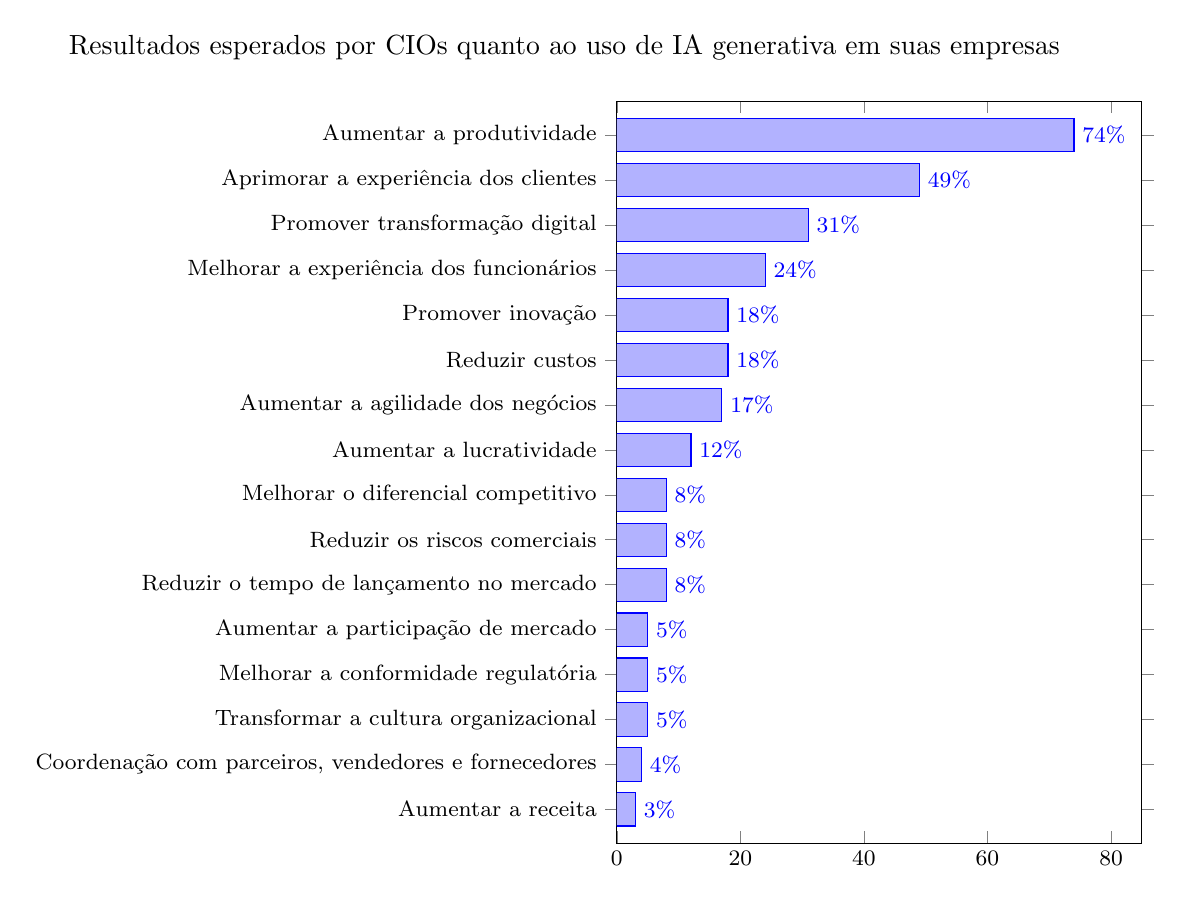
\begin{tikzpicture}
        \footnotesize
        \begin{axis}[
                xbar,
                width=8.25cm,
                height=11cm,
                title={Resultados esperados por CIOs quanto ao uso de IA generativa em suas empresas},
                title style={at={(-0.1,1.05)}, anchor=center, font=\normalsize},
                xmin=0,
                xmax=85,
                y dir=reverse,
                bar width=12pt,
                nodes near coords=\pgfmathprintnumber{\pgfplotspointmeta}\%,
                nodes near coords align={horizontal},
                enlarge y limits=0.05,
                symbolic y coords={
                        prod, clientes, digital, funcionarios, inovacao,
                        custos, agilidade, lucro, diferencial, riscos,
                        tempo, mercado, conformidade, cultura, parceiros, receita
                    },
                ytick=data,
                yticklabels={
                        Aumentar a produtividade,
                        Aprimorar a experiência dos clientes,
                        Promover transformação digital,
                        Melhorar a experiência dos funcionários,
                        Promover inovação,
                        Reduzir custos,
                        Aumentar a agilidade dos negócios,
                        Aumentar a lucratividade,
                        Melhorar o diferencial competitivo,
                        Reduzir os riscos comerciais,
                        Reduzir o tempo de lançamento no mercado,
                        Aumentar a participação de mercado,
                        Melhorar a conformidade regulatória,
                        Transformar a cultura organizacional,
                        {Coordenação com parceiros, vendedores e fornecedores},
                        Aumentar a receita
                    }
            ]

            \addplot coordinates {
                    (74,prod)
                    (49,clientes)
                    (31,digital)
                    (24,funcionarios)
                    (18,inovacao)
                    (18,custos)
                    (17,agilidade)
                    (12,lucro)
                    (8,diferencial)
                    (8,riscos)
                    (8,tempo)
                    (5,mercado)
                    (5,conformidade)
                    (5,cultura)
                    (4,parceiros)
                    (3,receita)
                };

        \end{axis}
    \end{tikzpicture}
\end{figure}

Quanto às previsões de adoção, a \emph{Gartner} indica uma forte tendência de adoção da IA agêntica nos próximos anos. Segundo o relatório, até 2028, 33\% dos aplicativos de \emph{software} empresariais incluirão IA agêntica, em comparação com menos de 1\% em 2024 e que, até 2028, pelo menos 15\% das decisões cotidianas no trabalho serão tomadas de forma autônoma por IAs agênticas, em comparação com 0\% em 2024.

Na figura \autoref{fig:gartner_cios}, o relatório compilou os resultados de uma pesquisa de opinião realizada com 78 CIOs de empresas, os quais foram perguntados "Quais são os três principais tipos de valor de negócios que sua empresa busca com a aplicação de IA generativa?". Com este gráfico e com os pontos levantados ao longo do relatório fica claro que o investimento das empresas em ferramentas de IA, em especial a agêntica, está fundamentalmente atrelado à crença de que a IA aumentará a produtividade dos funcionários. Ao mesmo tempo que o texto parece otimista em relação à adoção de IAs, ele destaca que esse movimento possui diversos riscos, os quais são vistos como responsabilidade das empresas usuárias mitigar.